\section{Fundamentals of Computer Security}
\label{sec:sec:fundamentals}

Above we specified that a defender must consider all system entries and all possible security holes.
The measures applied by a defender are preventive measures and reactive measures.
These efforts of a defender are permanent.
They cannot stop and say "done, I have secured the system."
The system must be continuously monitored and updated.
Moreover, given the frequent changes at the software level (new applications or new versions of applications), hardware (new systems, new processor-level functionalities), or infrastructure (higher speed connections, interconnection with services), the system is in continuous change.

We say that \textbf{security is a process, not an end goal}.
The efforts to secure a system are continuous efforts.
A developer, administrator, or designer of a system must consider its security as a permanent element of their activity, and their actions must maintain or increase the system's security.
Losing the security perspective during the design, development, or administration of a system can lead to increased security risks and system attacks.

The perspective of security as a process, as a continuous action, requires permanent resource allocation.
These resources can be physical resources (doors, locks, firewall devices), financial (acquisition of security software/hardware), human resources (competent people, security training), or process resources (procedures and security guidelines).
A system is more secure to the extent that more and higher quality resources are invested in its security.
An ordinary user will not invest many resources in security because their data and systems are not so interesting to an attacker.
A large company, especially a bank, will however need significant investments for security, being a much more likely target of attackers.

\subsection{Security Objectives}
\label{sec:sec:fundamentals:objectives}

To increase the security of a system means to eliminate, or better said, to hinder attacks.
The security of a system means achieving certain objectives for that system, objectives that are compromised in case of an attack.
Ideally, these objectives are achieved for all systems, but some may be prevalent for certain systems.
We present below the main security objectives, noting that they are not exhaustive and are not completely separate.

One of the most important objectives is \textbf{confidentiality}.
Confidentiality refers, in general, to stored data and transferred data.
We say that confidentiality is ensured if only authorized users or entities can access and view the data.
Confidentiality is generally ensured with the help of encryption, as we will clarify in \labelindexref{Section}{sec:sec:data:confidentiality}.

Another data-related objective is \textbf{integrity}.
If an attacker cannot view data (i.e., confidentiality is ensured), they can still modify the data;
we say that the attacker corrupts the data.
Data corruption can mean the loss of data for a victim entity or can mean inducing different behavior: the victim believes the data is correct and makes a different decision based on it.
Data integrity is generally ensured by hashing algorithms, as we will detail in \labelindexref{Section}{sec:sec:data:integrity}.

A secure system is a system that responds to user requests to obtain the desired results.
Therefore, an objective of security is \textbf{availability} (\textit{availability}).
Similar concepts are reliability (\textit{reliability}) and robustness (\textit{robustness}).
A system is available when it consistently provides the appropriate service to users, regardless of conditions.
That is, in case of a resource abuse attack such as DoS (\textit{Denial of Service}), the system functions within satisfactory parameters.
Ensuring the availability of a system depends on several measures, such as system monitoring, entry verification, redundancy, or hardware reliability.

An increasingly present objective in our days, dominated by social networks and users' virtual profiles, is \textbf{privacy protection} (\textit{privacy}).
The notion of privacy refers to protecting the personal aspects of an individual: personal data, photos, or relationships.
These are pieces of information that are not directly useful to others, but which can affect the person's personal or public profile.
Interest in privacy has grown as more companies profit from having access to users' private information, information that can be used abusively.
Measures for ensuring privacy protection are technical measures, such as access anonymization, reducing online presence, filling in online forms only with strictly necessary information, and legal measures, such as the "General Data Protection Regulation" (\textit{General Data Protection Regulation} - GDPR\abbrev{GDPR}{General Data Protection Regulation}) in the European Union\footnote{\url{https://gdpr-info.eu/}}.
Ensuring privacy is an important responsibility of every user.
To ensure that a person's private aspects are used non-abusively, that person must be continuously concerned about their online presence and the data they provide in the online environment.

\subsection{Security Notions}
\label{sec:sec:fundamentals:notions}

The two perspectives for security are the attacker's perspective and the defender's perspective.
The defender has access to the system and seeks to protect it.
The attacker seeks to abuse the system by bypassing the defender's protection measures.
It should be noted that the defender must protect the system against attacks, but also against inappropriate situations generated, without intention, by legitimate users.
An application can malfunction both due to an attack (with malicious intentions), but also due to unexpected usage (with legitimate intentions).

As we specified above, the attacker role can also be taken by someone with good intentions, who seeks to exploit a system to provide the necessary information and to help solve problems.
We call this type of role \textbf{white-hat hacker} or \textbf{ethical hacker}.
On the other hand, a malicious attacker is simply called an attacker, \textbf{cracker}, or \textbf{black-hat hacker}.

We say that a system has a \textbf{defect} (\textit{bug}, \textit{flaw}) if there is an unexpected situation that leads to the inadequate functioning of that system.
Such a bug can manifest during legitimate use.
We often talk about defects/bugs in applications: when we use a certain command or a sequence of actions, the application terminates its execution or generates inappropriate behavior.

A bug becomes a \textbf{vulnerability} when it can be exploited by an attacker.
Exploiting a vulnerability means that an attacker can use that vulnerability for their benefit.
A bug does not lead to personal benefit, but a vulnerability does.
For example, if an application displays, in case of an unexpected situation, random information, we say it is a bug;
however, if an application displays a list of passwords or private data, information that can be used by an attacker, then we say it is a vulnerability.

An \textbf{exploit} is a tool (which can be an application, input data, or a device) that can be used to exploit a vulnerability.

When an attacker knows of the presence of one or more vulnerabilities at the system level, they will attempt to exploit them seeking a benefit in the direction of those presented at the beginning of the chapter: gaining control, information theft, or resource abuse.
For this, an attacker builds an \textbf{attack vector}.
An attack vector represents the set of steps that an attacker follows to obtain a benefit in the attacked system.
Usually, a single vulnerability and, therefore, a single exploit are not sufficient, so the attacker will link multiple exploits into an attack vector.
For example, it can be an exploit to bypass a firewall, one to obtain a shell in a system, another to gain access to the password database, another to access a server and, from there, to obtain critical information.
In \labelindexref{Figure}{fig:sec:attack-vector} the idea of an attack vector is presented schematically.

\begin{figure}[htbp]
  \centering
  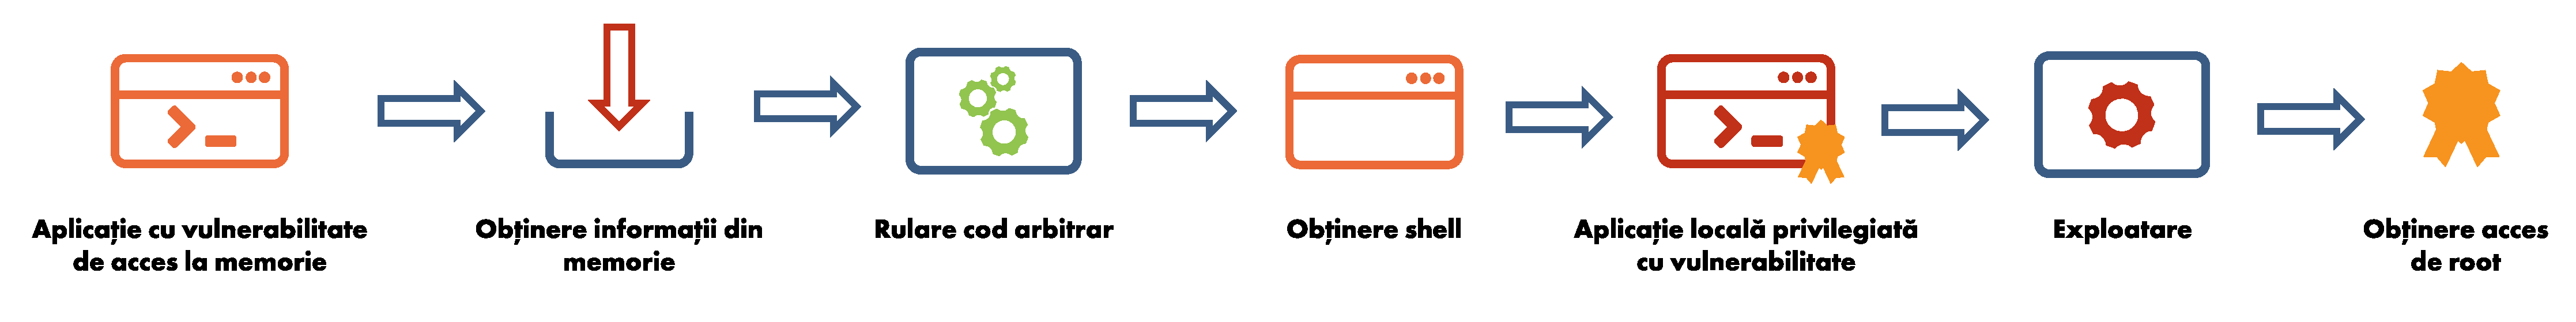
\includegraphics[width=\columnwidth]{chapters/12-auth/img/attack-vector.pdf}
  \caption{Attack Vector}
  \label{fig:sec:attack-vector}
\end{figure}

In their objective to obtain their own benefits, an attacker needs a way to access a system.
Nowadays, accessibility through the Internet means that many systems are attackable remotely.
The initial targets of attackers are the system entry points, that is, the ways in which a system can be accessed.
We say that the entries of a system represent the \textbf{attack surface} of a system (\textit{attack surface});
a system has a larger attack surface the more entries it has or the wider the entries are.
A large attack surface means high security risk.
So, one of the ways a defender protects the system is by reducing the attack surface.

The principle of reducing the attack surface also applies in another context.
A system has a critical component for proper functioning on which the entire system depends.
For example, on a regular computer system, this component is given by the operating system and the privileged services of the system.
When the operating system or a privileged service is compromised, equivalent to obtaining the \texttt{root} account in Linux or the \texttt{Administrator} account in Windows, we say that the entire system is compromised.
We call this critical component of the system \textbf{Trusted Computing Base} (TCB\abbrev{TCB}{Trusted Computing Base}), as we indicate in \labelindexref{Figure}{fig:sec:tcb}.
The TCB must be protected the most within the system.
Non-TCB components can be compromised without compromising the entire system, but compromising the TCB means compromising the system.
Given its relevance in system security, the size of the TCB must be as small as possible, that is, the TCB must have as reduced an attack surface as possible, reducing critical security risks.

\begin{figure}[htbp]
  \centering
  \def\svgwidth{\columnwidth}
  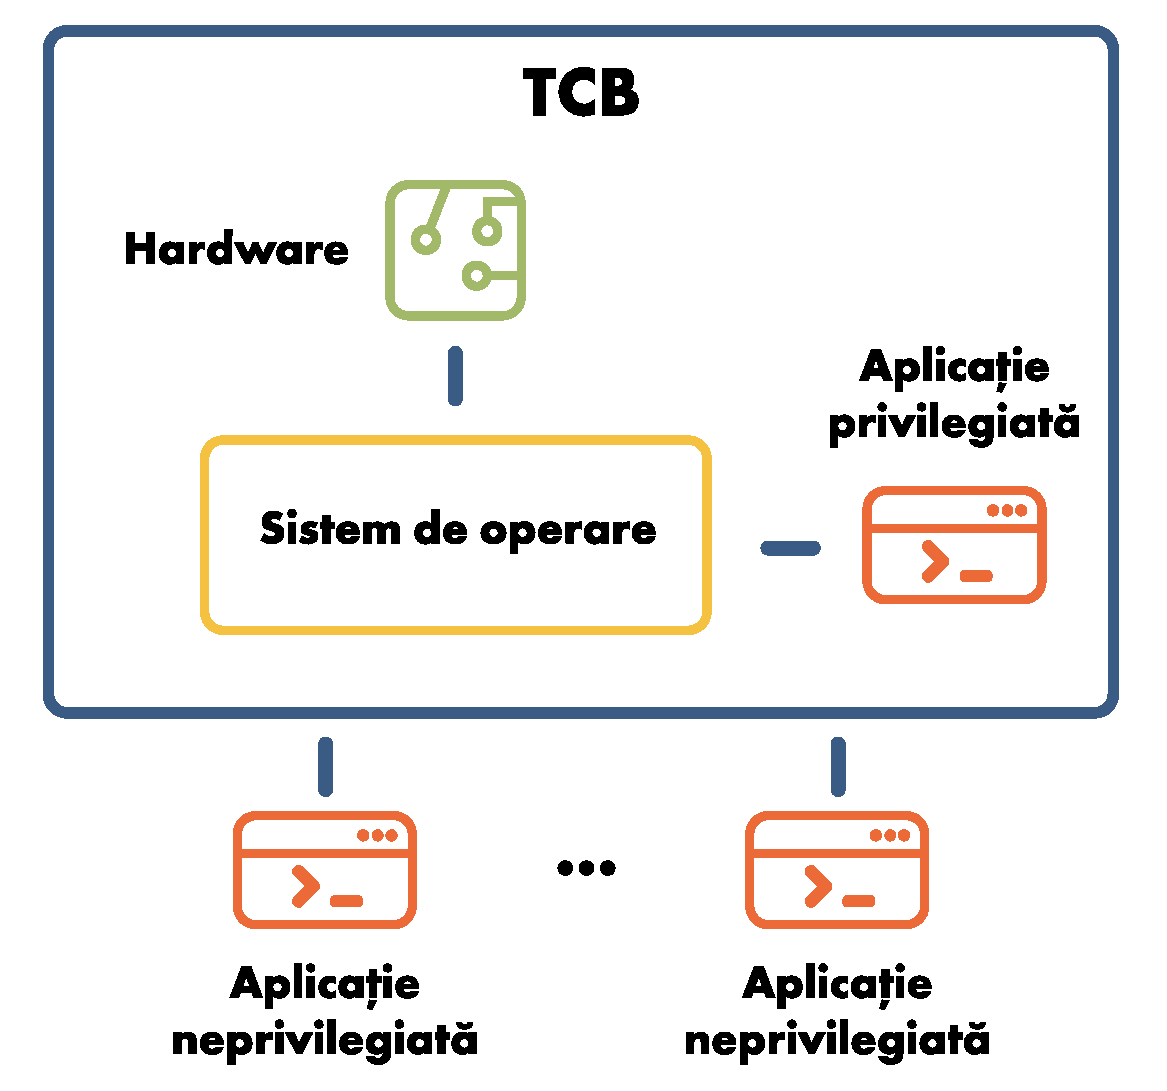
\includegraphics[width=0.7\textwidth]{chapters/12-auth/img/tcb.svg.pdf}
  \caption{Trusted Computing Base (TCB) in a computer system}
  \label{fig:sec:tcb}
\end{figure}

\subsection{Security Principles}
\label{sec:sec:fundamentals:principles}

In the design, development, and administration of a system, there are security principles that are recommended to be followed to minimize attack risks or damages caused by an attack.

One of the most important principles is the \textbf{principle of least privilege}.
A system has components (hardware, software, infrastructure) that interact with each other.
A certain component, for example a certain process, needs access to certain resources to function.
The principle of least privilege dictates that the implementation of security mechanisms should not allow the component access to other resources.
Thus, if an application is compromised, the impact of the damages produced will be minimal: only at the level of resources accessible to the application.

The principle of least privilege correlates with \textbf{modular system design}.
When the system is monolithic (has no clear separations between components), access to all resources is granted to the entire system.
When the system is modular, formed of multiple parts, each part is assigned the minimum necessary set of privileges: one part has access to certain resources, another part to other resources, limiting the potential damages in case of compromise of one part.
We can say that the principle of least privilege, together with modular design, leads to reducing the impact surface in case of an attack.
In \labelindexref{Figure}{fig:sec:modular-vs-monolithic} the difference between a monolithic system design and a modular one and the benefit of using the principle of least privilege is specified.

\begin{figure}[htbp]
  \centering
  \def\svgwidth{\columnwidth}
  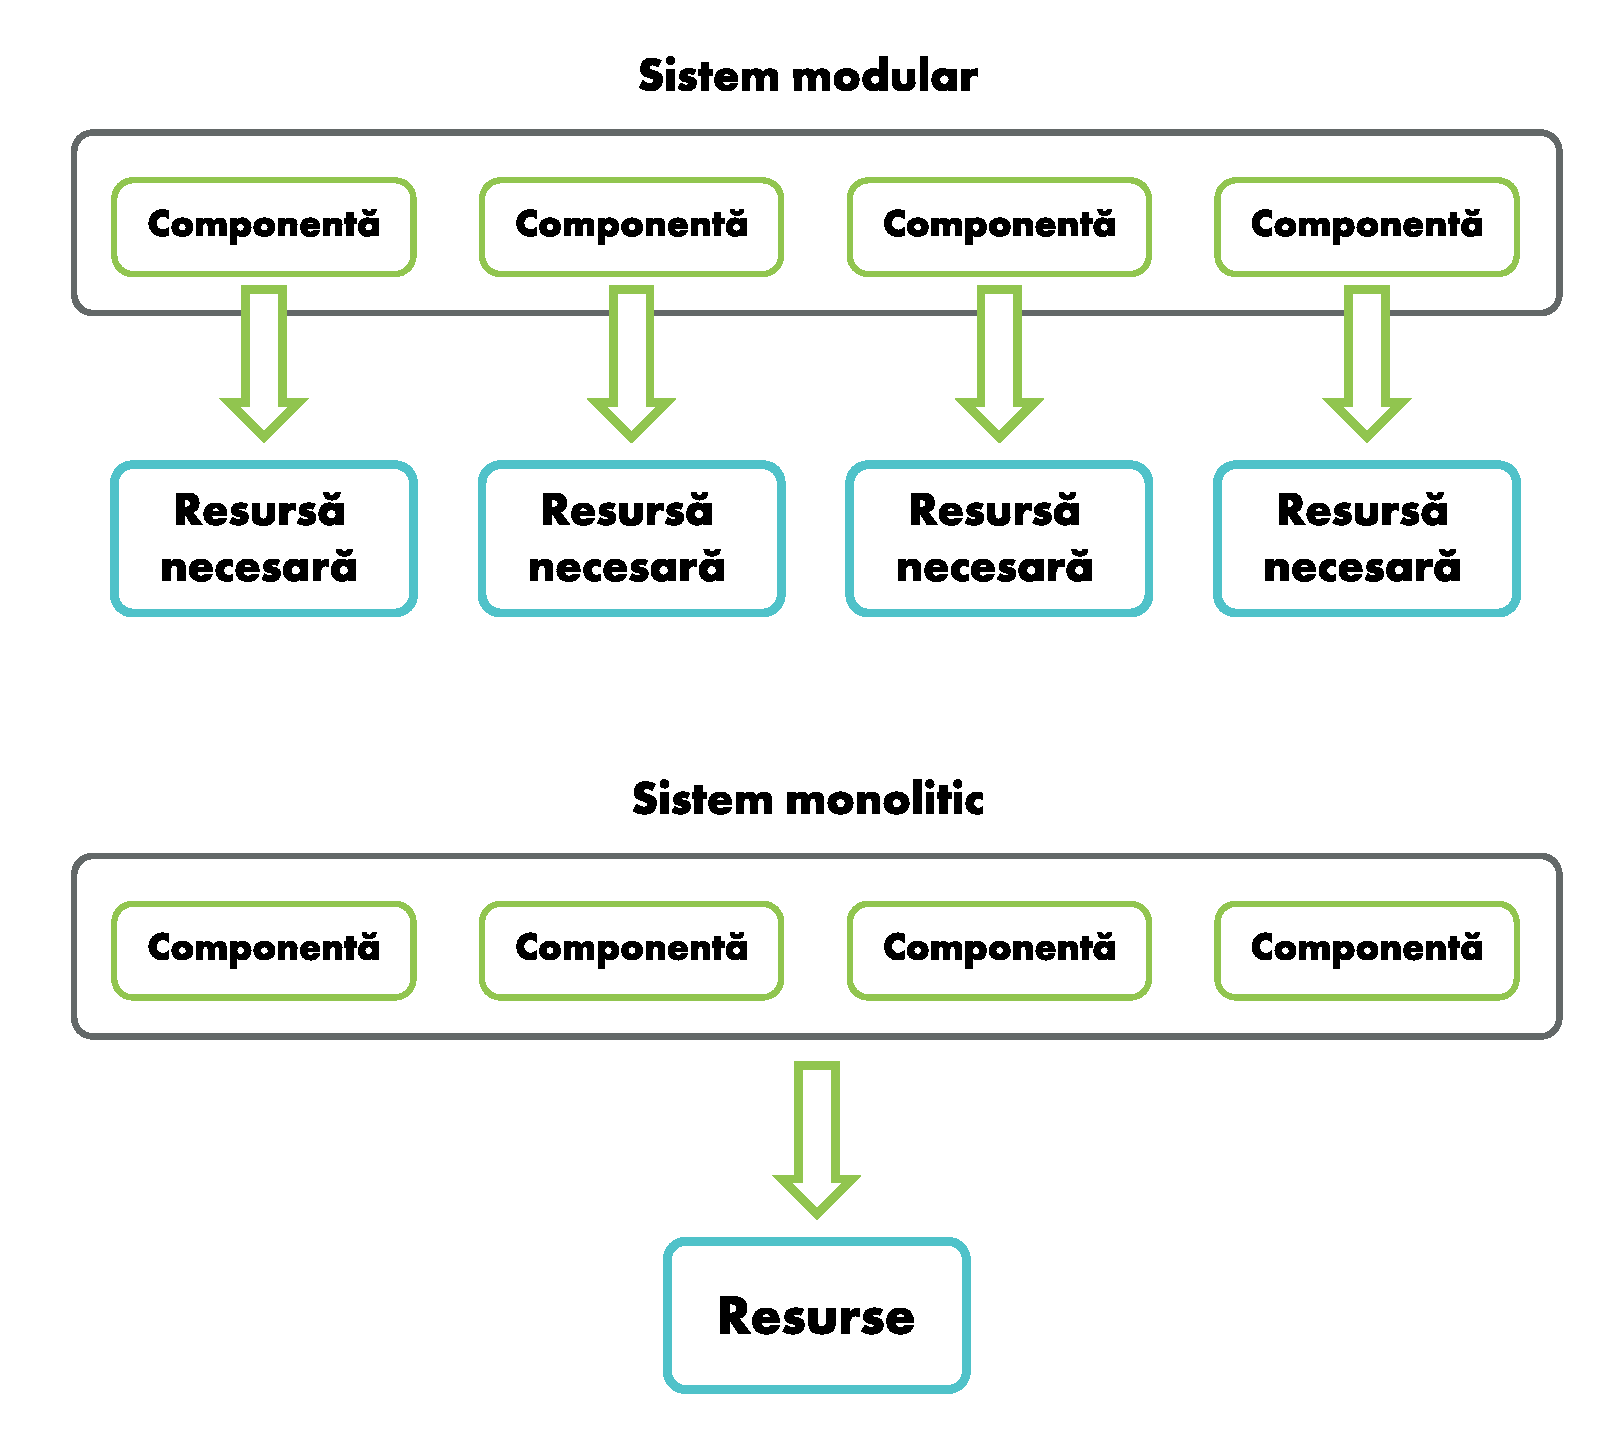
\includegraphics[width=0.7\textwidth]{chapters/12-auth/img/modular-vs-monolithic.svg.pdf}
  \caption{Resource access in a monolithic and modular system}
  \label{fig:sec:modular-vs-monolithic}
\end{figure}

The defensive means that can be used in securing a system are not infallible.
For increasing the security of a system, the \textbf{principle of defense in depth} or \textbf{multi-layer defense} (\textit{defense in depth}, \textit{multi-layer security}) is recommended with multiple defensive means present simultaneously in securing a system.
These means are complementary, similar to multiple defensive walls: penetrating one defensive means places the attacker in front of another defensive means, making it difficult to create an attack vector capable of defeating all means.

In system design, the attacker's perspective must be continuously considered.
An attacker will try to find the simplest way to access and control or abuse the system.
We call the \textbf{weakest link} (\textit{weakest link}) the component that has a high level of vulnerability.
This will be the preferred target of attackers and its compromise leads, in general, to the compromise of a large part of the system.
An attacker can start from a small breach in the system and can expand it, through consecutive exploits, until the compromise of the entire system.
Modularization and the principle of least privilege help isolate damages, while securing components and ensuring an adequate security level for the weakest link reduces the risk of an attack occurring.

When securing a system is desired, we make the \textbf{separation between security policy and security mechanism} (\textit{security policy}, \textit{security mechanism}).
The policy refers to security rules and principles, described conceptually.
The mechanism refers to effective implementations, specific to the system, that satisfy the rules and principles.
The principle of separating mechanism from policy is important to allow the implementation of different mechanisms or multiple mechanisms for the same policy.
Changing the mechanism does not affect the policy, and those who decide the policy do not need to have internal details related to the mechanism, thus focusing on the conceptually important part.

\subsection{Subject-Object Model.
Access Permissions}
\label{sec:sec:fundamentals:permissions}

In implementing security principles, systems and the interaction between their components are described by the \textbf{subject-object model} (\textit{subject-object model}).
In this model, the subject, also called agent, is the active entity, the entity that executes actions.
The object, also called resource, is the passive entity, the entity upon which actions are executed.
The security of a system is given by the access rules of subjects to objects.
A subject \texttt{S1} can have write access to object \texttt{O1}, subject \texttt{S2} can have read access to object \texttt{O1}, and subject \texttt{S3} may not have access to any resource.
These rules are generally represented in graph form as in \labelindexref{Figure}{fig:sec:access-permissions}.

\begin{figure}[htbp]
  \centering
  \def\svgwidth{\columnwidth}
  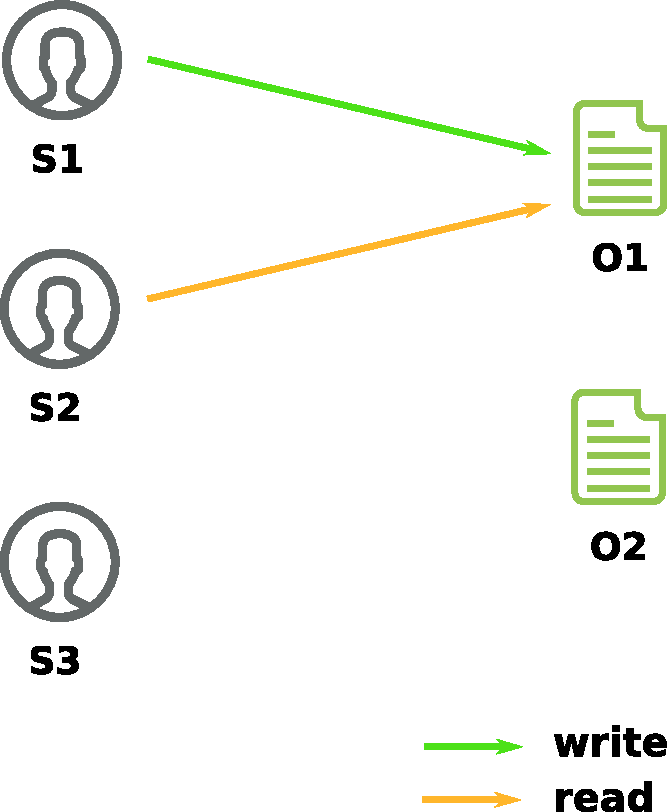
\includegraphics[width=0.4\textwidth]{chapters/12-auth/img/access-permissions.svg.pdf}
  \caption{Access Permissions}
  \label{fig:sec:access-permissions}
\end{figure}

A privileged entity, which is part of the system's TCB, also called \textbf{reference monitor} (\textit{reference monitor}) is the one that allows or denies subjects' access to objects.
For this, access permissions are configured that establish for each subject and object what permissions each has.
The way in which the reference monitor manages subjects' access to objects is described in \labelindexref{Figure}{fig:sec:reference-monitor}.
Most often, the reference monitor is the operating system.

\begin{figure}[htbp]
  \centering
  \def\svgwidth{\columnwidth}
  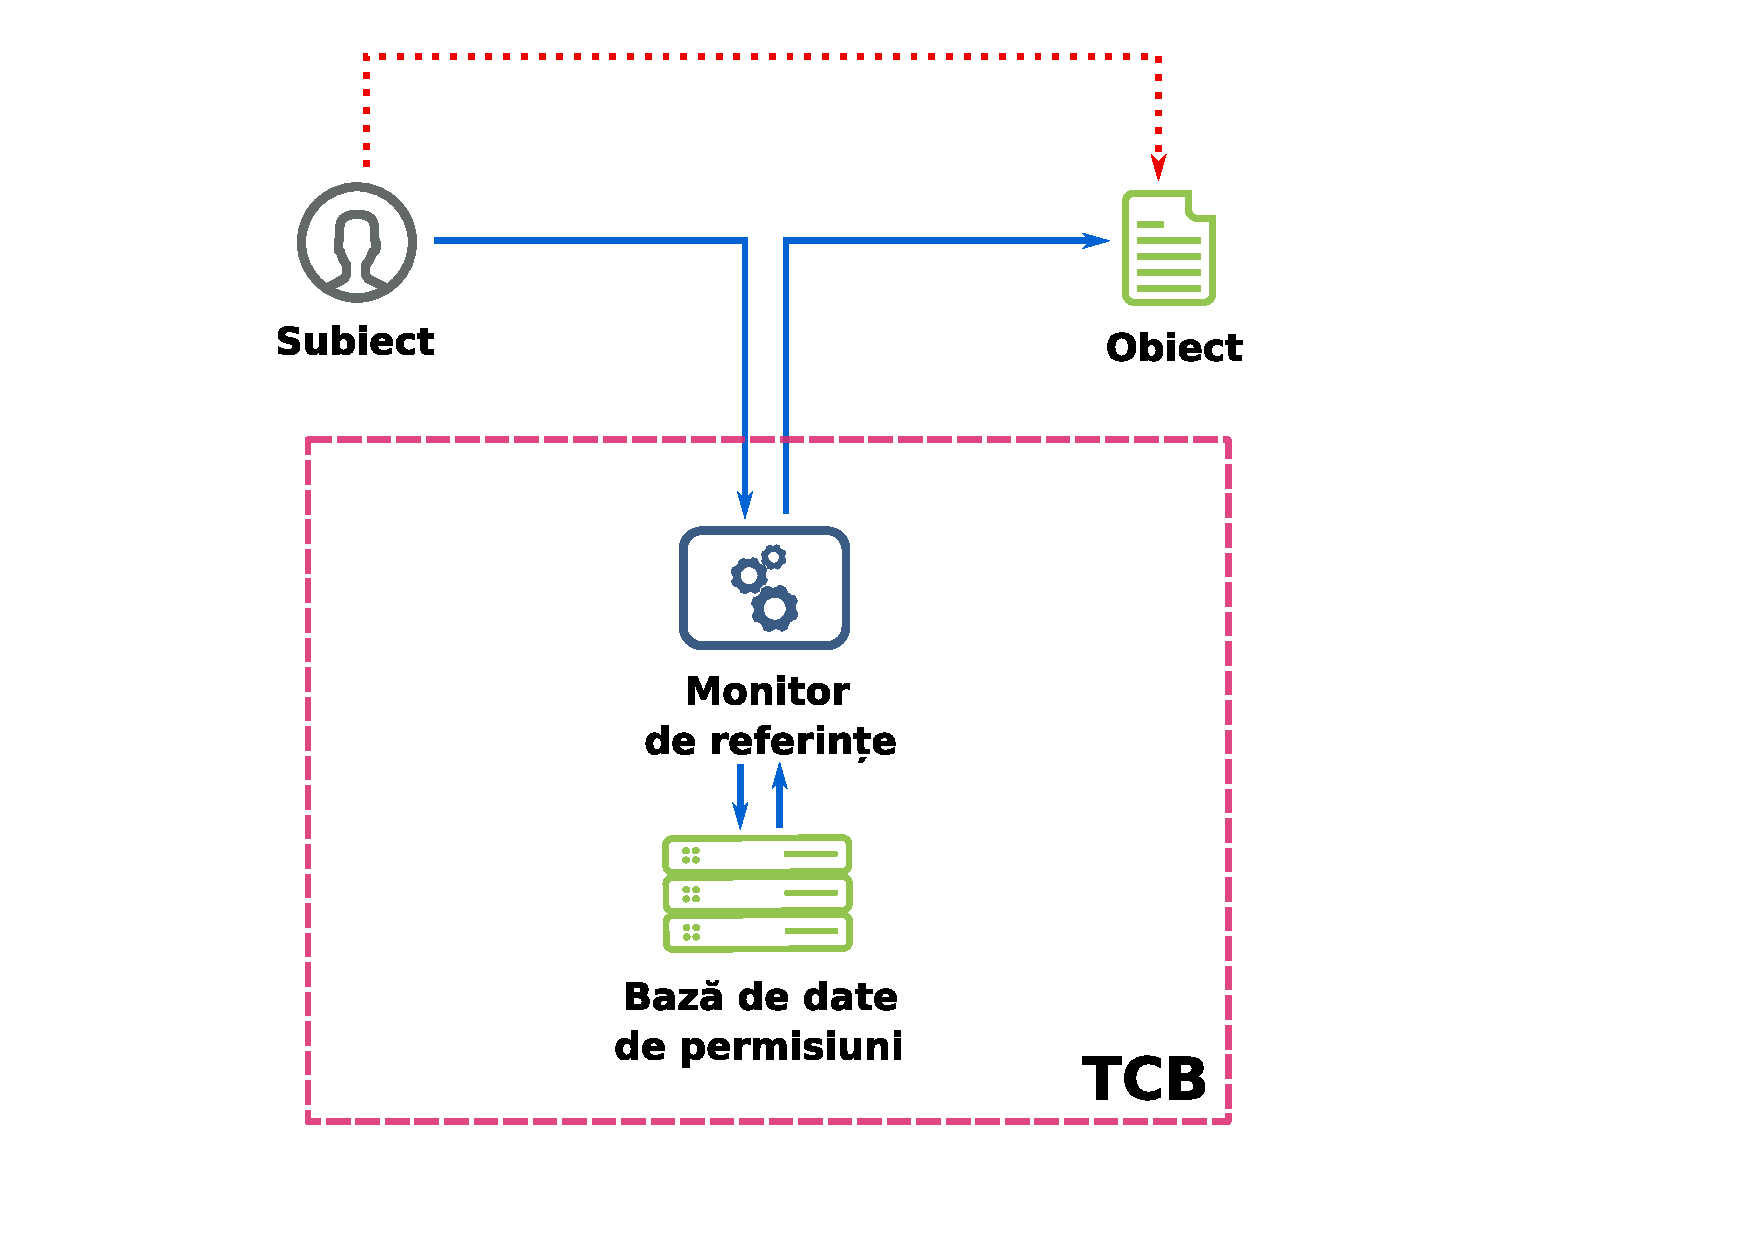
\includegraphics[width=0.5\textwidth]{chapters/12-auth/img/reference-monitor.svg.pdf}
  \caption{Reference Monitor (reference monitor)}
  \label{fig:sec:reference-monitor}
\end{figure}

A form of implementation of the subject-object model is represented by permissions in the file system which we will discuss in \labelindexref{Section}{sec:sec:data:fs}.
In this case, the subject is the process, and the object is the file that is desired to be accessed.
Within the file are stored the access permissions based on which the reference monitor (i.e., the operating system) provides access.
The subject-object model is simplified in the case of file system permissions: there are no entries for each subject (process) but they are aggregated into the three classes of entities: user (\textit{user}), group (\textit{group}), others (\textit{others}).

In the context of the subject-object model, we speak of the three types of related actions: authentication, authorization, and access control.

\textbf{Authentication} is the action through which a subject is identified in the system.
At that moment, there is an identification element (\textit{authentication token}) known to the system.
An example is password-based authentication through which a user can create processes with a certain user identifier (UID).
After authentication, the subject can access objects.

The subject's access to the object is conditioned by the permissions database that associates a subject with an object and with access permissions.
Completing an entry in this permissions database, that is, adding a new permission for a subject to an object is called \textbf{authorization} (\textit{authorization}).
Revoking authorization (\textit{unauthorizing}) is the inverse operation, of removing a permission.
In Linux, authorization in the file system is performed by the utilities \cmd{chmod} and \cmd{chown}.

When a subject seeks to access a resource, access is validated by the reference monitor by consulting the permissions database.
This consultation and allowing or denying access is called \textbf{access control} (\textit{access control}).
Access control occurs, in Linux, when running any command that accesses a file in one form or another: \cmd{cat}, \cmd{ls}, \cmd{vim}. 